\documentclass[11pt,a4paper]{article}

% Packages
\usepackage[utf8]{inputenc}
\usepackage[spanish, es-tabla, es-lcroman]{babel}
\usepackage{caption}
\usepackage{listings}
\usepackage{adjustbox}
\usepackage[shortlabels]{enumitem}
\usepackage{boldline}
\usepackage{amssymb, amsmath}
\usepackage[margin=1in]{geometry}
\usepackage{xcolor, color}
\usepackage{soul}
\usepackage{epstopdf}
\usepackage{hyperref}
\hypersetup{
     colorlinks   = true,
}

% Meta
\title{\textbf{ESTRUCTURA DE DATOS}\\
	   \textit{Práctica 1. Eficiencia de algoritmos}\\
	   \large \vspace{0.25em} Doble Grado de Informática y Matemáticas}
\author{Víctor Castro Serrano\\ Maximino Suárez van Gelderen}
\date{\today}

% Custom
\providecommand{\abs}[1]{\lvert#1\rvert}
\setlength\parindent{0pt}
\definecolor{Light}{gray}{.90}
\definecolor{mygreen}{rgb}{0,0.6,0}
\definecolor{mygray}{rgb}{0.5,0.5,0.5}
\definecolor{mymauve}{rgb}{0.58,0,0.82}
\renewcommand\labelenumi{(\emph{\roman{enumi})}}
\newcommand{\bm}[1]{\boldsymbol{#1}}

\lstset{literate=   % listings config
  {á}{{\'a}}1 {é}{{\'e}}1 {í}{{\'i}}1 {ó}{{\'o}}1 {ú}{{\'u}}1
  {Á}{{\'A}}1 {É}{{\'E}}1 {Í}{{\'I}}1 {Ó}{{\'O}}1 {Ú}{{\'U}}1
  {à}{{\`a}}1 {è}{{\`e}}1 {ì}{{\`i}}1 {ò}{{\`o}}1 {ù}{{\`u}}1
  {À}{{\`A}}1 {È}{{\'E}}1 {Ì}{{\`I}}1 {Ò}{{\`O}}1 {Ù}{{\`U}}1
  {ä}{{\"a}}1 {ë}{{\"e}}1 {ï}{{\"i}}1 {ö}{{\"o}}1 {ü}{{\"u}}1
  {Ä}{{\"A}}1 {Ë}{{\"E}}1 {Ï}{{\"I}}1 {Ö}{{\"O}}1 {Ü}{{\"U}}1
  {â}{{\^a}}1 {ê}{{\^e}}1 {î}{{\^i}}1 {ô}{{\^o}}1 {û}{{\^u}}1
  {Â}{{\^A}}1 {Ê}{{\^E}}1 {Î}{{\^I}}1 {Ô}{{\^O}}1 {Û}{{\^U}}1
  {œ}{{\oe}}1 {Œ}{{\OE}}1 {æ}{{\ae}}1 {Æ}{{\AE}}1 {ß}{{\ss}}1
  {ű}{{\H{u}}}1 {Ű}{{\H{U}}}1 {ő}{{\H{o}}}1 {Ő}{{\H{O}}}1
  {ç}{{\c c}}1 {Ç}{{\c C}}1 {ø}{{\o}}1 {å}{{\r a}}1 {Å}{{\r A}}1
  {€}{{\EUR}}1 {£}{{\pounds}}1 {ñ}{{\~{n}}}1
}

\lstset{    %listings config
  language=C++,
  belowcaptionskip=1\baselineskip,
  breaklines=true,
  frame=L,
  xleftmargin=0.5in,
  %otherkeywords={},
  showstringspaces=false,
  backgroundcolor=\color{white},
  basicstyle=\footnotesize\ttfamily,
  keywordstyle=\bfseries\color{purple!90!black},
  commentstyle=\itshape\color{gray!85!},
  identifierstyle=\color{blue!80!black},
  stringstyle=\color{green!60!black},
}

\newcommand\ddfrac[2]{\frac{\displaystyle #1}{\displaystyle #2}}

% Environments

\begin{document}
\maketitle

\section*{Condiciones de ejecución.}

Dado que en los siguientes ejercicios hablaremos de la eficiencia de distintos programas, conviene detallar las condiciones en las que se han llevado a cabo las pruebas. \\

\textbf{Hardware:} Asus GL552VW, Intel Core i5-6300HQ CPU @ 2.30GHz 4 cores, Intel HD Graphics 530 (Skylake GT2), 12GB RAM. \\
\textbf{Sistema Operativo:} Ubuntu 16.04.3 LTS 64-bit. \\
\textbf{Compilador:} g++ \\
\textbf{Opciones de compilación:} -g -o


\section*{Ejercicio 3.}

\textbf{a)} En este primer apartado, describiremos el funcionamiento del algoritmo proporcionado en el archivo $ejercicio\_desc.cpp$.\\

Se trata de un algoritmo de \textbf{búsqueda binaria}, donde dado un vector $v$ de $n$ elementos enteros, busca el entero $x$ en él. Para ello, se pasan como parámetros el inicio \textit{(inf)} y el final (\textit{sup}) de dicho vector. La función devuelve la posición donde se ha encontrado el elemento, o $-1$ si no estaba en el vector.\\

Para el correcto funcionamiento del algoritmo, es imprescindible que el vector esté \textbf{ordenado}, pues el procedimiento es el siguiente:

\begin{enumerate}
\item Se establece la posición $med = (inf+sup)/2$.
\item Se comprueba si el elemento $x$ está en la posición $med$.
\item Si está, hemos acabado. Si no está, se comprueba si el elemento $v[med]$ es mayor o menor que $x$.
    \begin{itemize}
    \item Si $v[med] < x$, actualizamos $inf = med + 1$.
    \item Si $v[med] > x$, actualizamos $sup = med - 1$.
    \end{itemize}
\item Repetimos el proceso, hasta encontrar el elemento, o concluir que no está en el vector.
\end{enumerate}

En resumen, el procedimiento se basa en dividir el vector original por la mitad, y si no está ahí el elemento buscado, nos quedamos únicamente con el sub-vector donde se puede encontrar dicho elemento (recordemos que el vector está ordenado). Repitiendo el proceso, acabaremos encontrando el elemento, o descubriendo que no está en el vector, cuando ya no se puedan hacer más divisiones.\\

\textbf{b)} Para el cálculo de la eficiencia teórica de la \textit{búsqueda binaria}, nos basamos en el hecho de que se divide sucesivamente en dos un vector de tamaño $n$. En el caso peor, el proceso continuará hasta que no se puedan hacer más divisiones del vector.\\

Como el resto de operaciones son elementales ($O(1)$), concluímos que la eficiencia del algoritmo es logarítmica, es decir, $T(n) \in O(\log (n))$. \\

\textbf{c)} Algunas ejecuciones tardan 0 segundos, suponemos que es porque el elemento se encontraba en el medio del vector.  Para solucionar el problema, ejecutamos el mismo algoritmo muchas veces (en nuestro caso, 10000000) y dividimos el tiempo total de ejecución entre el numero de ejecuciones. Los datos se ven reflejados en \textit{tiempos\_binario\_medio.dat} cuya grafica es la siguiente: \\


\begin{center}
	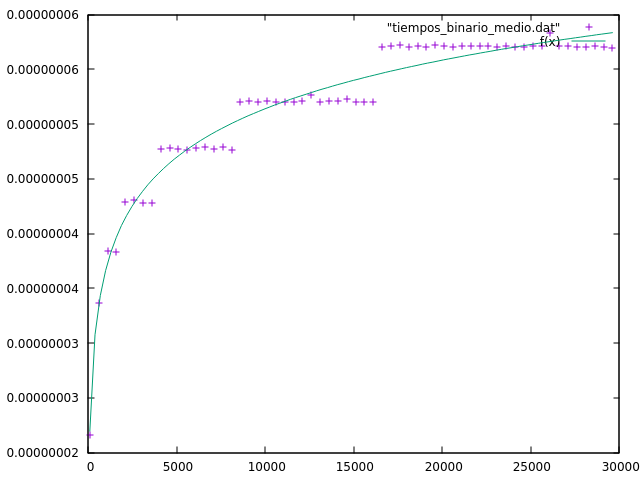
\includegraphics[height=10cm]{graficaej3.png}
\end{center}

Ajustando la nube de puntos a la función exponencial $f(x) = {6.40319 \cdot 10^{-09}log (x) - 2.57655 \cdot 10^{-09}}$ , se puede observar claramente que la eficiencia empírica describe una gráfica de forma logarítimica, coincidiendo así con nuestros resultados teóricos.

\end{document}
